Comminication between two agents can be modelled as a simple sender-receiver model~\cite{Crawford1998ATalk}. 



\begin{figure}[H]
	\centering
	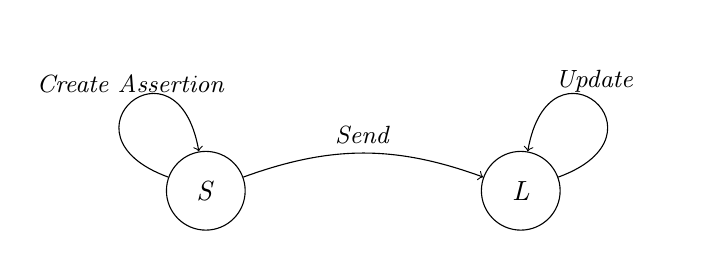
\begin{tikzpicture}[baseline=(S.base)]
		\tikzset{every loop/.style={min distance=10mm,looseness=10}}
		\node (S) at (0, 0) [shape=circle,draw,minimum size=1cm] {\textit{S}};
		\node (L) at (4, 0) [shape=circle,draw, minimum size=1cm] {\textit{L}};
		\path[->] (S) edge[bend left = 20] node[above]{\small \textit{Send}} (L)
		edge[loop above,in=100,out=160, min distance=8mm,looseness=8] node{\small \textit{Create Assertion}} (S)
		(L) edge[loop above,in=80,out=20, min distance=8mm,looseness=8] node{\small \textit{Update}} (L);
	\end{tikzpicture}
	\caption{Simple model of the interaction between two agents. \textit{S} is the speaker and \textit{L} is the listener. \textit{S} creates an argument that it then sends to \textit{L}. \textit{L} will then update its own beliefs according to the argument it receives from \textit{S}.}
	\label{fig:simple_interaction}
\end{figure}

A general form of this interaction has a sender/speaker, shown as \textit{S} in \cref{fig:simple_interaction}, communicating with a receiver/listener shown as \textit{L}. In  this model there are two parts that could be varied. The method by which the speaker creates the assertion and the update rule with which the listener updates its beliefs given the assertion. Here we assume that the speaker has access to information about the listener, such as its beliefs and its update rule. 